\chapter{Изучение поглощения света в полупроводниках}

\section{Цель работы}
Целью работы является изучения основных механизмов поглощения света в полупроводниках и освоение методики исследований спектров поглощения света в полупроводниках в видимой и ближней инфракрасной области спектра.

\section{Теоретическая часть}
\subsection{Коэффициент поглощения света}
Если поток фотонов с длиной волны $\lambda$ и интенсивностью $I_{0}(\lambda)$ падает на плоскопараллельный образец толщиной $d$, то можно исследовать интенсивность отражённого от поверхности образца света $I_{R}(\lambda)$ и определить безразмерный коэффициент отражения

\begin{equation}
R(\lambda) = \frac{I_{R}(\lambda)}{I_{0}(\lambda)}
\end{equation}

а также измерить интенсивность прошедшего через образец света $I_{T}(\lambda)$ и определить безразмерный коэффициент пропускания

\begin{equation}
T(\lambda) = \frac{I_{T}(\lambda)}{I_{0}(\lambda)}
\end{equation}

Интенсивность прошедшего через образец света однозначно определяется коэффициентом отражения, поглощением внутри образца и отражением от внутренних граней. Закон Бугера-Ламберта внутри образца, на поверхность которого падает свет выглядит следующим образом:

\begin{equation}
I(x, \lambda) = I_{0}(\lambda) \left[ 1 - R(\lambda) \right] \exp{(- \alpha (\lambda) x )}
\end{equation}
где $\alpha(\lambda)$ - коэффициент поглощения, имеет размерность обратной длины.

Величина $\alpha^{-1}$ определяет толщину кристалла, проходя через которую свет ослабляется в $e$ раз. Это значит, что можно считать величину $\alpha$ вероятностью поглощения фотона на единице длины. Если имеется несколько независимых механизмов поглощения света в кристалле, то полный коэффициент поглощения будет суммой коэффициентов, определяемых каждым механизмом независимо.

\begin{equation}
\alpha(\lambda) = \sum\limits_{i}{\alpha_{i}(\lambda)}
\label{eq6_alphasum}
\end{equation}

Зависимость $\alpha(\lambda)$ называется спектром поглощения для данного вещества.

Практическое использование формулы Бугера-Ламберта приводит к известным проблемам, связанным с невозможностью прямого измерения интенсивности света внутри кристалла на определённой глубине. При измерении интенсивности света, прошедшего через образец толщиной $d$ необходимо учитывать не только поглощение света данным слоем, но также долю отражённого света и сумму всех потоков с учётом многократного отражения. Сумму всех потоков можно представить в виде бесконечной геометрической прогрессии, первый член которой равен $I_{0} (1-R)^2 \exp(-\alpha d)$, а множитель $R^2 \exp(-2 \alpha d)$. Интенсивность света, прошедшего через образец $I_{T}$, таким образом находится как

\begin{equation}
I_{T} = I_{0} \frac{(1-R)^2 \exp(-\alpha d)}{1 - R^2 \exp(-2 \alpha d)}
\end{equation}

Если учесть, что обычно $\alpha d \gg 1$, в знаменателе можно пренебречь вторым членом и считать

\begin{equation}
I_{T} = I_{0} (1-R)^2 \exp(-\alpha d)
\end{equation}

Откуда можно получить коэффициент поглощения на данной длине волны:

\begin{equation}
\alpha = \frac{1}{d} \ln \frac{I_{0} (1-R)^2}{I_{T}}
\label{eq6_alpha_T}
\end{equation}

Если неизвестен коэффициент отражения, то величину $\alpha$ можно определить, сравнивая интенсивность света, прошедшего через два образца из одного материала с одинаковой обработкой поверхностью, но различной толщины. В таком случае для образцов с толщинами $d_{1}$ и $d_{2}$

\begin{equation}
\alpha = \frac{1}{d_{1}-d_{2}} \ln \frac{I_{T1}}{I_{T2}}
\end{equation}

\subsection{Механизмы поглощения света}
Основные механизм поглощения света в полупроводниках определяются возможными типами переходов носителей заряда между зонами, или типами возбуждаемых светом тепловых колебаний решётки кристалла (фононов). Электронные и дырочные механизмы поглощения схематически показаны на рисунке \ref{pic6_transition}.

\begin{figure}[h!]\centering
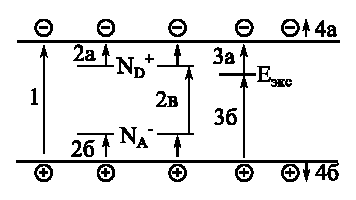
\includegraphics{pic6_transition.eps}
\caption{Схема электронных переходов при различных механизмах поглощения света}
\label{pic6_transition}
\end{figure}

На рисунке обозначены:

\begin{enumerate}
\item Собственное или фундаментальное поглощение света, связанное с переходом электрона из валентной зоны в зону проводимости.
\item примесное поглощение, связанное с переходами электронов с примесного уровня в зону проводимости (2а на рисунке), из валентной зоны на примесный уровень (2б) или между различными примесными центрами (2в).
\item Экситонное поглощение, связанное с возбуждением экситона (переход 3б) или распадом на пару электрон-дырка (3а).
\item Поглощение свободными носителями заряда, сопровождаемое переходом свободных носителей на более высокие энергетические состояния внутри зоны.
\item Фононное поглощение (на рисунке не может быть отражено), связанное с возбуждением в кристалле одного или нескольких фононов - квантов тепловых колебаний решётки.
\end{enumerate}

Рассмотрим форму спектра поглощения для каждого из механизмов по отдельности.

\paragraph{Собственное поглощение}
Рассмотрим поглощение фотона с энергией $E_{\text{ф}} = \hbar \omega$ непрямозонным полупроводником с шириной запрещённой зоны $E_{g} < E_{\text{ф}}$. Пусть зонная структура имеет вид, приведённый на рисунке \ref{pic6_zone}.

\begin{figure}[h!]\centering
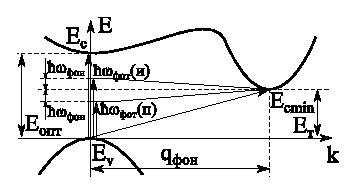
\includegraphics{pic6_zone.eps}
\caption{Схема непрямых переходов электронов при собственном поглощении}
\label{pic6_zone}
\end{figure}

Поглотив фотон, электрон переходит из валентной зоны в зону проводимости. Такие переходы могут происходить как прямым образом (практически без изменения волнового вектора электрона), так и непрямыми (между экстремумами разрешённых зон $E_{c}$ и $E_{v}$). Непрямые переходы требуют значительного изменения волнового вектора электрона.

Можно записать законы сохранения энергии и импульса для прямых переходов

\begin{equation}
E_{1} + \hbar \omega = E_{2}
\end{equation}

\begin{equation}
\overrightarrow{P_{1}} + \hbar \overrightarrow{q} = \overrightarrow{P_{2}}
\end{equation}
где $E_{1}$ и $E_{2}$ - энергии начального и конечного состояния электрона, $\overrightarrow{P_{1}} = \hbar \overrightarrow{k_{1}}$ и $\overrightarrow{P_{2}} = \hbar \overrightarrow{k_{2}}$ - квазиимпульсы электрона в начальном и конечном состоянии. Импульс поглощенного фотона составляет $\hbar \overrightarrow{q}$.Энергия фотона ограничена снизу величиной $\hbar \omega_{min} = E_{g}$, что соответствует длине волны фотона $\lambda_{max} = \frac{\hbar c}{E_{g}}$, где $c$ - скорость света. Если измерять длину волны в микрометрах, а ширину запрещённой зоны в электрон-вольтах, то подставляя известные значения получим удобную формулу:

\begin{equation}
\lambda = \frac{1.24}{E_{g}}
\label{eq6_homega}
\end{equation}

Например, для GaAs ширина запрещённой зоны составляет 1.4 эВ, что соответствует длине волны 0.9 мкм. Значение волнового вектора для фотона с такой энергией составляет:

\begin{equation}
|\overrightarrow{q}| = \frac{2 \pi}{\lambda} \approx 7 \cdot 10^{4}  \text{см}^{-1}
\end{equation}

Волновой вектор электрона можно оценить по формуле

\begin{equation}
|\overrightarrow{k}| = \sqrt{\frac{2 m^{*} k_{0} T}{\hbar^{2}}}
\end{equation}
где $m^{*}$ - эффективная масса электрона, $k_{0}$ - константа Больцмана, $T$ - температура.

При комнатной температуре значение волнового вектора электрона $|\overrightarrow{k}| \approx 10^{7} \text{см}^{-1}$, что значительно больше волнового вектора фотона. Таким образом, в выражении для закона сохранения импульса можно пренебречь импульсом фотона и записать:

\begin{equation}
\overrightarrow{P_{1}} = \overrightarrow{P_{2}}
\end{equation}

или, что то же самое,

\begin{equation}
\overrightarrow{k_{1}} = \overrightarrow{k_{2}}
\end{equation}

Из-за того,что такие переходы идут без изменения волнового вектора, они и названы прямыми.

Спектр поглощения для прямых разрешённых переходов имеет вид

\begin{equation}
\alpha(\hbar \omega) \sim (\hbar \omega - E_{g})^{\frac{1}{2}}
\end{equation}

В свою очередь, для прямых запрещённых переходов

\begin{equation}
\alpha(\hbar \omega) \sim (\hbar \omega - E_{g})^{\frac{3}{2}}
\end{equation}

Суммарный спектр поглощения представляет собой сумму этих двух, а значит при $\hbar \omega \gtrapprox E_{g}$ можно считать, что зависимость коэффициента поглощения определяется только разрешёнными переходами. Если экспериментальные данные спектра вблизи края собственного поглощения построить в координатах $\alpha^2 = f(\hbar \omega)$, то должна получиться прямая линия, точка пересечения которой с осью абсцисс даёт значение ширины запрещённой зоны для прямых переходов (см. рисунок \ref{pic6_direct}).

\begin{figure}[h!]\centering
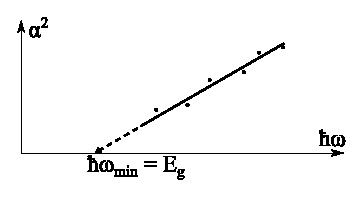
\includegraphics{pic6_direct.eps}
\caption{Представление спектра поглощения для определения ширины запрещённой зоны при прямых переходах}
\label{pic6_direct}
\end{figure}

Для представленного на рисунке \ref{pic6_zone} материала <<оптическая>> ширина запрещённой зоны $E_{\text{опт}}$ оказывается больше, чем минимальная ширина, определяемая как разность между дном зоны проводимости и потолком валентной зоны: $E_{g} = E_{c min} - E_{v}$. Эта величина называется термической шириной запрещённой зоны, так как она определяет термическую активацию электронов в собственном полупроводнике.

В непрямозонном полупроводнике оптические переходы между $E_{c}$ и $E_{v}$ также возможны, но они должны идти при значительном изменении волнового вектора электрона. Так, в Si точки экстремума $E_{v}$ соответствуют центру зоны Бриллюэна, т.е. $|\overrightarrow{k}| = 0$, а для $E_{c}$ находятся вблизи границы в направлении $(100)$, что соответствует $|\overrightarrow{k}| \approx 10^8 \text{см}^{-1}$. Изменение волнового вектора электрона, таким образом, много больше волнового вектора фотона, участвующего в поглощении. Поэтому в процессе поглощения должна использоваться третья частица, волновой вектор которой может достигать подобных значений. Такими частицами в данном случае выступают фононы - кванты тепловых колебаний решётки. Их энергия составляет $\hbar \omega_{\text{фон}} \approx 10^{-2}$ эВ, а волновой вектор $|\overrightarrow{q}| \le 10^{8} \text{см}^{-1}$. Непрямые межзонные оптические переходы могут идти как с поглощением, так и с испусканием фонона. Законы сохранения энергии и импульса для таких переходов будут иметь вид:

\begin{equation}
E_{1} + \hbar \omega_{\text{фот}} \pm \hbar \omega_{\text{фон}} = E_{2}
\end{equation}

\begin{equation}
\overrightarrow{P}_{1} + \hbar \overrightarrow{q}_{\text{фот}} \pm \hbar \overrightarrow{q}_{\text{фон}} = \overrightarrow{P}_{2}
\end{equation}
здесь индексы <<фот>> и <<фон>> относятся к фотону и фонону соответственно. Величиной $\hbar \overrightarrow{q}_{\text{фот}}$ можно пренебречь. Знак минус говорит о процессе испускания фонона, знак плюс - о поглощении.

Спектр поглощения для непрямых переходов описывается следующим образом:

\begin{equation}
\alpha(\hbar \omega_{\text{фот}}) =
C_{1} \frac{\left[ \hbar \omega_{\text{фот}} - (E_{g}-\hbar \omega_{\text{фон}}) \right]^{2}}{\exp \left( \frac{\hbar \omega_{\text{фон}}}{k_{0} T} \right) - 1} +
C_{2} \frac{\left[ \hbar \omega_{\text{фот}} - (E_{g}+\hbar \omega_{\text{фон}}) \right]^{2}}{1 - \exp \left( -\frac{\hbar \omega_{\text{фон}}}{k_{0} T} \right)}
\end{equation}
здесь первый член описывает процессы, связанные с поглощением фононов, второй - с испусканием.

На рисунке \ref{pic6_nondirect} показан спектр поглощения для непрямозонного полупроводника вблизи края собственного поглощения.

\begin{figure}[h!]\centering
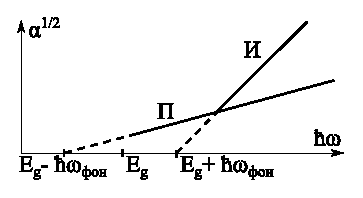
\includegraphics{pic6_nondirect.eps}
\caption{Определение ширины запрещённой зоны и энергии фононов по спектрам поглощения при непрямых переходах}
\label{pic6_nondirect}
\end{figure}

Продолжение участков <<И>> и <<П>> до пересечения с осью абсцисс даст пороговые энергии фотонов для процессов поглощения света, сопровождаемых испусканием и поглощением фонона ($\hbar \omega_{\text{фот}} = E_{g} + \hbar \omega_{\text{фон}}$ и $\hbar \omega_{\text{фот}} = E_{g} - \hbar \omega_{\text{фон}}$) соответственно. Очевидно, значение термической ширины запрещённой зоны $E_{g}$ может быть получено как среднее между этими двумя значениями.

Также в непрямозонном полупроводнике будет наблюдаться поглощение, связанное с прямыми переходами, но оно будет сдвинуто в область более высоких энергий фотонов.

\paragraph{Экситонное поглощение света}
Экситоны - это возбуждённые состояния собственных атомов, которые могут быть представлены в водородоподобной модели как связанная пара электрон-дырка, вращающаяся относительно центра масс. В этой модели эффективная масса экситона $m_{ex}^{-1} = (m_{n}^{-1} + m_{p}^{-1})$. Энергия экситонных состояний равна $E_{ex} = 13.6 \frac{m_{ex}}{m_{0}} \frac{1}{\varepsilon^2} \frac{1}{n^2}$.

Оптические переходы электронов из валентной зоны на экситонные состояния с различными индексами $n$ должны отличаться по энергиям поглощенных фотонов. Так, для уровней 1 и 2:

\begin{equation}
\begin{split}
\hbar \omega_{2} - \hbar \omega_{1} &= \left( E_{g} - E_{ex}(2) \right) - \left( E_{g} - E_{ex}(1) \right) \\
&= E_{ex}(1) -  E_{ex}(2) =  E_{ex}(1) \cdot \left( 1 - \frac{1}{4} \right) \\
&= \frac{3}{4} E_{ex}(1)
\end{split}
\end{equation}

Тогда можно записать:

\begin{equation}
\begin{split}
E_{ex}(1) &= \frac{4}{3} (\hbar \omega_{2} - \hbar \omega_{1}) \\
E_{g} &= \hbar \omega_{1} + E_{ex}(1) = \hbar \omega_{1} + \frac{4}{3} (\hbar \omega_{2} - \hbar \omega_{1})
\end{split}
\end{equation}

На рисунке \ref{pic6_exiton} показан вид экситонного спектра поглощения и диаграмма электронных переходов при оптическом возбуждении экситонов. Экситонные линии спектра расположены вблизи края собственного поглощения. Экситонные состояния заметны лишь в достаточно чистых кристаллах при низких температурах.

\begin{figure}[h!]\centering
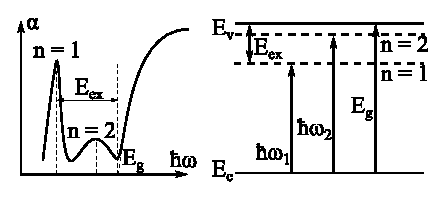
\includegraphics{pic6_exiton.eps}
\caption{Экситонное поглощение света}
\label{pic6_exiton}
\end{figure}

\paragraph{Примесное поглощение света}
Оптическая ионизация примесных центров в полупроводниках связана с переходом электрона из валентной зоны на акцепторный уровень или с донорного уровня в зону проводимости. Энергия фотона, поглощённого при таком переходе, может быть больше или равна энергии ионизации примеси.

Легирующие примеси дают мелкие примесные уровни в запрещённой зоне, и поэтому для их оптической ионизации нужны небольшие энергии: $\hbar \omega \ge 10^{-2}$ эВ, что соответствует далёкой инфракрасной области спектра. Глубокие примесные центры требуют для оптической ионизации гораздо больших энергий. Также возможны переходы с ионизированных примесных состояний в разрешённые зоны - так называемые переходы <<примесь - дальняя зона>>. Так, например, при переходе электрона с акцепторного уровня в зону проводимости, пороговые энергии квантов будут лишь ненамного отличаться от необходимой для собственной ионизации, так как $E_{g} \gg E_{a}-E_{v}$. Таким образом, примесное поглощение, связанное с оптической ионизацией мелких примесей, даёт полосы поглощения в дальней инфракрасной области, а примесное поглощение, связанное с оптической нейтрализацией ионизированных примесных центров, даёт полосы, накладывающиеся на спектр собственного поглощения и создающие <<хвосты>> поглощения при энергиях $\hbar \omega < E_{g}$.

\paragraph{Поглощение света свободными носителями заряда}
Свободные электроны в зоне проводимости, как и свободные дырки в валентной зоне, могут при поглощении света полупроводником переходить внутри своих разрешённых зон в более высокие энергетические состояния. Так как спектр энергий внутри разрешённых зон можно считать непрерывным, то носители могут поглощать фотоны с непрерывно меняющейся энергией, и структурных особенностей для такого спектра наблюдаться не будет. Классическая теория даёт для коэффициента поглощения света свободными носителями заряда следующую зависимость:

\begin{equation}
\alpha(\lambda) = \frac{n e^2 \lambda^2}{8 \pi^2 \tilde{n} c^3 \tau(\overrightarrow{k}) m^{*}}
\label{eq6_nonsel}
\end{equation}
где $\tilde{n}$ - показатель преломления в материале.

Таким образом, коэффициент поглощения растёт по параболическому закону с увеличением длины волны поглощаемых фотонов, и тем больше, чем больше концентрация свободных носителей заряда $n$. Переходы свободных носителей в разрешённых зонах при поглощении фотона оказываются непрямыми, и поэтому для соблюдения законов сохранения импульса и энергии требуют участия ещё одной частицы. Учёт конкретных механизмов рассеяния при поглощении света свободными носителями заряда даёт зависимости $\alpha(\lambda)$ в виде:

\begin{itemize}
\item $\alpha(\lambda) \sim \lambda^{3/2}$ для рассеяния на акустических фононах;
\item $\alpha(\lambda) \sim \lambda^{5/2}$ для рассеяния на оптических фононах;
\item $\alpha(\lambda) \sim \lambda^{7/2}$ для рассеяния на ионах примеси;
\end{itemize}

Анализируя спектр поглощения света в области поглощения свободными носителями можно определить концентрацию свободных носителей и доминирующий механизм рассеяния.

При сложной структуре разрешённых зон возможен не только внутризонный механизм поглощения света, но и поглощение, связанное с переходами между состояниями в различных подзонах в пределах данной разрешённой зоны энергий. Так, например, на рисунке \ref{pic6_subzone} показаны оптические переходы свободных дырок между подзонами тяжёлых (1), лёгких (2) и средних (3) дырок, которые могут происходить в германии и кремнии, а также спектр поглощения при таких переходах. На спектре появляется характерная структура в виде края (1-2) и двух максимумов (2-3 и 1-3). По положению минимума между двумя максимумами можно определить энергию спин-орбитального расщепления $E_{so}$ между подзоной средних дырок и точкой $E_{v max}$ - потолком валентной зоны. Такой характерный спектр поглощения носит название селективного поглощения свободными носителями заряда, в отличие от неселективного, описываемого формулой (\ref{eq6_nonsel}). Этот механизм может наблюдаться также для электронов в зоне проводимости, если зона проводимости имеет сложную структуру в виде частично перекрывающихся подзон энергии.

\begin{figure}[h!]\centering
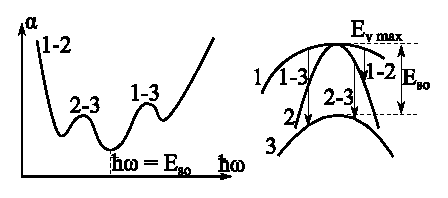
\includegraphics{pic6_subzone.eps}
\caption{Селективное поглощение света свободными дырками}
\label{pic6_subzone}
\end{figure}

\paragraph{Поглощение света тепловыми колебаниями решётки}
Поглощать световую энергию могут не только свободные и связанные электроны и дырки, но и атому кристаллической решётки. При этом в кристалле возникают дополнительные кванты тепловых колебаний решётки, т.е. фононы. Такое поглощение может быть как однофононным (рождение в кристалле одного фонона при поглощении одного фотона), так и многофононным (рождение в кристалле двух и более фононов при поглощении одного фотона). В силу законов сохранения при однофононным поглощении света могут возникать только поперечные оптические фононы (т.к. фотон - квант поперечного электромагнитного поля). Такое поглощение имеет специфический остро резонансный характер, так как в каждом кристалле может с некоторой максимальной вероятностью возникать только вполне определённый тип поперечных оптических фононов. Коэффициент поглощения света при однофононном поглощении весьма велик у кристаллов с большой долей ионной связи. Так как кристаллы сильно отражают свет в той области, где велико его поглощение, то в спектре отражения ионных кристаллов наблюдается резонансный пик отражения света, связанный с однофононным поглощением. Это отражение получило название <<явления остаточных лучей>> и использовалось в спектроскопии для монохроматизации света в ИК-области спектра.

В полупроводниках с большой долей ковалентных связей наблюдается преимущественно многофононное поглощение света решёткой кристалла. При этом поглощённый фотон порождает в кристалле вполне определённый набор комбинаций фононов. Например, $LO + 2 TA$ - продольный оптический и два поперечных акустических фонона. Такие наиболее вероятные комбинации фононов дают острые пики в спектре поглощения света в далёкой ИК-области. Характеристические спектры решёточного многофононного поглощения накладывается обычно на спектр поглощения свободными носителями заряда, который также даёт существенный вклад в далёкой ИК-области спектра.

\paragraph{Общий спектр поглощения света}
В силу соотношения (\ref{eq6_alphasum}), общий спектр поглощения для данного образца может быть получен как сумма спектров каждого отдельного механизма. Общая картинка спектра в широком диапазоне длин волн может иметь вид, представленный на рисунке \ref{pic6_spectrum}.

\begin{figure}[h!]\centering
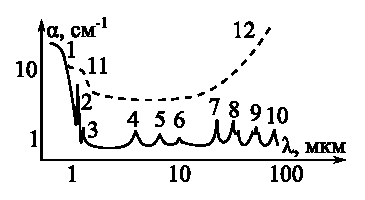
\includegraphics{pic6_spectrum.eps}
\caption{Общий вид спектра поглощения света в полупроводниках. Сплошная линия - слаболегированный, пунктирная - сильнолегированный материал. 1 - край собственного поглощения; 2,3 - экситоны и экситонно-примесные комплексы; 4,5,6 - примесное поглощение; 7,8,9,10 - многофононное поглощение; 11 - сдвиг края собственного поглощения в сильнолегированном образце; 12 - неселективное поглощение свободными носителями.}
\label{pic6_spectrum}
\end{figure}

В коротковолновой части спектра лежит край собственного поглощения, вблизи которого может наблюдаться характерная структура экситонного спектра. В области более длинных волн за краем собственного поглощения могут наблюдаться примесные полосы поглощения, соответствующие глубоким примесным центрам. Поглощение свободными носителями заряда монотонно растёт с длиной волны в ИК-области спектра. На него накладывается характерная структура многофононного решёточного поглощения света. Вид спектра поглощения кристалла существенно зависит от концентрации примесей в полупроводнике. При возрастании концентрации легирующей примеси растёт поглощение на свободных носителях заряда (в длинноволновой области), пропадает экситонная структура вблизи края собственного поглощения, сам край собственного поглощения может сдвигаться в коротковолновую область за счёт эффекта Бурштейна-Мосса.

\section{Методика измерений и описание установки}
Для определения спектра поглощения $\alpha(\lambda)$ требуется знать коэффициент пропускания $T(\lambda)$, толщину образца $d$ и коэффициент отражения $R(\lambda)$. В данной работе можно считать коэффициент отражения равным нулю, а коэффициент поглощения таков, что $\alpha d < 1$, что позволяет воспользоваться достаточно простой формулой (\ref{eq6_alpha_T}).

Блок-схема установки приведена на рисунке \ref{pic6_scheme}.

\begin{figure}[h!]\centering
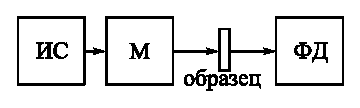
\includegraphics{pic6_scheme.eps}
\caption{Блок-схема измерительной установки. Здесь ИС - источник света с фокусирующей системой, М - монохроматор, ФД - фотодатчик с регистрирующим устройством.}
\label{pic6_scheme}
\end{figure}

В ходе работы из непрерывного спектра, даваемого источником, необходимо выделять отдельные длины волн. Для этого используется универсальный монохроматор УМ-2. В качестве источника сплошного спектра принимается отверстие в полости с температурой $T$, которую имитирует лампа накаливания с температурой нити 3000 К. Разложение непрерывного спектра производится при помощи призмы, при этом длина волны, подаваемая на выход монохроматора, определяется углом поворота призмы. Угол может плавно меняться вращением барабана. При работе с монохроматорами такого рода необходима градуировка, которая позволит поставить в соответствие углу поворота призмы длину волны, получаемую на выходе. Для градуировки используется ртутная лампа, в спектре которой наблюдаются яркие полосы. Длины волн некоторых линий спектра ртути приведены в таблице \ref{table6_Hg}.

\begin{table}[h!]
\caption{Длины волн некоторых линий спектра ртути}
\begin{center}
\begin{tabular}{c|c|c}
Цвет & Длина волны, нм & Угол поворота барабана \\
\hline
Глубокий красный & 730 & \\
Красный & 623 & \\
Красный & 619 & \\
Оранжевый & 607 & \\
Желтый & 579 & \\
Желтый & 576 & \\
Зелёный & 546 & \\
Голубой & 491 & \\
Синий & 435 & \\
Фиолетовый & 408 & \\
Фиолетовый & 404 & \\
\hline
\end{tabular}
\end{center}
\label{table6_Hg}
\end{table}

Образец для измерения спектра поглощения должен иметь вид тонкой плоскопараллельной пластины с отполированными поверхностями. Держатель для образца имеет вид шторки с двумя прорезями, в одну из которых вставляется образец. Коэффициент пропускания на данной длине волны определяется как отношение интенсивности света прошедшего через образец к интенсивности света, прошедшего через незакрытую прорезь в шторке: $T(\lambda) = I_{\text{обр}}(\lambda)/I_{\text{0}}(\lambda)$.

Интенсивность выходного сигнала определяется как величина, пропорциональная выходному сигналу фотодетектора $U$. Выходной сигнал снимается универсальным вольтметром В7-16А.

\section{Порядок проведения работы и указания по технике безопасности}

\begin{enumerate}
\item Произвести градуировку монохроматора, для чего 
	\begin{enumerate}
	\item установить на рельс ртутную лампу, включить блок питания и дать ей прогреться;
	\item установить необходимый размер входной щели и фокусировку линзы для визуального различения жёлтого дуплета ртути;
	\item выводить поочерёдно спектральные линии ртути и фиксировать в таблице \ref{table6_Hg} показания барабана поворотного устройства призмы монохроматора.
	\end{enumerate}
\item Произвести измерение пропускания $T(\lambda)$ образца, для чего
	\begin{enumerate}
	\item установить на рельс лампу накаливания и включить блок питания, сфокусировать световое пятно на входной щели монохроматора;
	\item установить шторку с прорезью перед выходной щелью;
	\item установить фотодетектор за выводной щелью;
	\item плавно вращая барабан монохроматора, фиксировать различие в выходном сигнале фотодетектора при пропускании света через прорезь без образца и через образец;
	\item Внести результаты измерений в таблицу \ref{table6_data}
	\end{enumerate}
\item Построить спектр поглощения образца в осях $\alpha^2 = f(\hbar \omega)$ и $\alpha^{1/2} = f(\hbar \omega)$. Сравнивая графики, сделать выводы о прямозонности материала.
\end{enumerate}

\begin{table}[h!]
\caption{Спектр поглощения образца}
\begin{center}
\begin{tabular}{c|c|c|c|c|c}
Угол & $\lambda$ & $U_{0}$ & $U_{\text{обр}}$ & T & $\alpha$ \\
\hline
 & нм & мВ & мВ &  & $\text{см}^{-1}$ \\
\hline
\end{tabular}
\end{center}
\label{table6_data}
\end{table}

Соблюдается стандартная техника безопасности при обслуживании высокоточных (до 3 А) источников. В ходе работы используются яркие лампы, на которые не рекомендуется смотреть невооружённым глазом.

\section{Обработка результатов эксперимента}
\begin{enumerate}
\item По линейной интерполяции данных таблицы \ref{table6_Hg} определяется формула пересчёта угла поворота призмы в длину волны в виде $y = a x + b$, где $y$ - длина волны, $x$ - угол.
\item По полученной формуле значения угла пересчитываются в энергию фотона с учётом соотношения (\ref{eq6_homega}).
\item Для прямозонного материала ширина запрещённой зоны определяется по линейной экстраполяции коэффициента поглощения на ось абсцисс в координатах $\alpha^2 = f(\hbar \omega)$, как это показано на рисунке \ref{pic6_direct}.
\item Для непрямозонного материала ширина запрещённой зоны определяется по экстраполяциям линейных участков, как это показано на рисунке \ref{pic6_nondirect}.
\item Исходя из полученной ширины запрещённой зоны делается вывод о том, какой материал был использован в данной работе.
\end{enumerate}

\section{Контрольные вопросы}
\begin{enumerate}
\item Понятие коэффициента поглощения. Размерность и порядок этой величины для полупроводников.
\item Как связаны величины $T$, $R$ и $\alpha$.
\item Основные механизмы поглощения света в полупроводниках.
\item Общий вид спектра поглощения и влияние на него легирующих примесей.
\item Вид спектра собственного поглощения и методы его анализа для прямых и непрямых переходов.
\item Определение ширины запрещённой зоны по краю собственного поглощения.
\item Факторы, влияющие на положение края собственного поглощения.
\item Экситонный спектр поглощения.
\item Почему экситонный спектр не наблюдается в поглощении при комнатной температуре, а также при высокой степени легирования образца?
\item Примесное поглощение света в полупроводниках.
\item Поглощение света тепловыми колебаниями решётки.
\item Механизмы поглощения света свободными носителями заряда.
\item Учёт влияния многократного отражения на измерение коэффициента поглощения.
\item Принцип работы монохроматора.
\end{enumerate}

\section{Литература}
\begin{enumerate}
\item П.С. Киреев. Физика полупроводников. СПб.: Лань, 2011 г.
\item В.В. Батавин, Ю.А. Концевой, Ю.В. Федорович. Измерение параметров полупроводниковых материалов и структур. М.: Радио и связь, 1985 г.
\item В.Н. Мартынов, Г.И. Кольцов. Полупроводниковая оптоэлектроника. М.: МИСИС, 1999 г.
\item В.В. Горбачев, Л.Г. Спицина. Физика полупроводников и металлов. М.: Высшая школа, 1986 г.
\end{enumerate}